\documentclass[11pt,a4paper]{article}
\usepackage[utf8]{inputenc}
\usepackage[italian]{babel}
\usepackage{geometry}
\usepackage{graphicx}
\usepackage{booktabs}
\usepackage{longtable}
\usepackage{hyperref}
\usepackage{xcolor}
\usepackage{enumitem}
\usepackage{fancyhdr}

\geometry{margin=2.5cm}

\hypersetup{
    colorlinks=true,
    linkcolor=blue,
    filecolor=magenta,      
    urlcolor=cyan,
    pdftitle={Documentazione Database KARIS},
    pdfauthor={Tommaso Caputi, Di Pasquale Giulio, Gadaleta Giovanni}
}

\pagestyle{fancy}
\fancyhf{}
\fancyhead[L]{Documentazione Database - KARIS}
\fancyhead[R]{\thepage}
\fancyfoot[C]{}

\title{Documentazione Database - KARIS}
\author{Tommaso Caputi, Di Pasquale Giulio, Gadaleta Giovanni}

\begin{document}

\maketitle
\newpage

\tableofcontents
\newpage

\section{Introduzione}

Il database \textbf{KARIS} è progettato per gestire la distribuzione di beni e risorse tra parrocchie, beneficiari e famiglie. Il sistema supporta la gestione di inventari, assegnazioni, richieste e inviti per utenti con diversi ruoli.

\textbf{Tecnologia}: PostgreSQL \\
\textbf{Encoding}: UTF-8 \\
\textbf{Tipi di dati}: Utilizzo di UUID per le chiavi primarie

\section{Schema Logico}

\subsection{parrocchia}
Rappresenta le parrocchie che utilizzano il sistema.

\begin{longtable}{p{3cm}p{3cm}p{4cm}p{5cm}}
\toprule
\textbf{Campo} & \textbf{Tipo} & \textbf{Vincoli} & \textbf{Descrizione} \\
\midrule
\endfirsthead
\toprule
\textbf{Campo} & \textbf{Tipo} & \textbf{Vincoli} & \textbf{Descrizione} \\
\midrule
\endhead
\bottomrule
\endfoot
\bottomrule
\endlastfoot
\texttt{id} & UUID & PRIMARY KEY, DEFAULT uuid\_generate\_v4() & Identificatore univoco \\
\texttt{nome} & TEXT & NOT NULL & Nome della parrocchia \\
\texttt{via} & TEXT & NULL & Indirizzo \\
\texttt{citta} & TEXT & NULL & Città \\
\texttt{piva} & TEXT & NULL & Partita IVA \\
\texttt{created\_at} & TIMESTAMP WITH TIME ZONE & DEFAULT now() & Data di creazione \\
\end{longtable}

\subsection{utente}
Rappresenta gli utenti del sistema (amministratori e volontari).

\begin{longtable}{p{3cm}p{3cm}p{4cm}p{5cm}}
\toprule
\textbf{Campo} & \textbf{Tipo} & \textbf{Vincoli} & \textbf{Descrizione} \\
\midrule
\texttt{id} & UUID & PRIMARY KEY, DEFAULT uuid\_generate\_v4() & Identificatore univoco \\
\texttt{nome} & TEXT & NOT NULL & Nome dell'utente \\
\texttt{cognome} & TEXT & NOT NULL & Cognome dell'utente \\
\texttt{cf} & TEXT & UNIQUE & Codice fiscale \\
\texttt{tipo\_utente\_id} & UUID & FOREIGN KEY $\rightarrow$ tipo\_utente(id) & Tipo di utente \\
\texttt{parrocchia\_id} & UUID & FOREIGN KEY $\rightarrow$ parrocchia(id) & Parrocchia di appartenenza \\
\texttt{created\_at} & TIMESTAMP WITH TIME ZONE & DEFAULT now() & Data di creazione \\
\end{longtable}

\subsection{tipo\_utente}
Definisce i tipi di utente disponibili nel sistema.

\begin{longtable}{p{3cm}p{3cm}p{4cm}p{5cm}}
\toprule
\textbf{Campo} & \textbf{Tipo} & \textbf{Vincoli} & \textbf{Descrizione} \\
\midrule
\texttt{id} & UUID & PRIMARY KEY, DEFAULT uuid\_generate\_v4() & Identificatore univoco \\
\texttt{descrizione} & TEXT & NOT NULL & Descrizione del tipo (es. "Amministratore", "Volontario") \\
\end{longtable}

\subsection{beneficiario}
Rappresenta le persone che ricevono aiuti dalla parrocchia.

\begin{longtable}{p{3cm}p{3cm}p{4cm}p{5cm}}
\toprule
\textbf{Campo} & \textbf{Tipo} & \textbf{Vincoli} & \textbf{Descrizione} \\
\midrule
\texttt{id} & UUID & PRIMARY KEY, DEFAULT uuid\_generate\_v4() & Identificatore univoco \\
\texttt{nome} & TEXT & NOT NULL & Nome del beneficiario \\
\texttt{cognome} & TEXT & NOT NULL & Cognome del beneficiario \\
\texttt{cf} & TEXT & UNIQUE & Codice fiscale \\
\texttt{data\_nascita} & DATE & NULL & Data di nascita \\
\texttt{luogo\_nascita} & TEXT & NULL & Luogo di nascita \\
\texttt{famiglia\_id} & UUID & FOREIGN KEY $\rightarrow$ famiglia(id) & Famiglia di appartenenza \\
\texttt{parrocchia\_id} & UUID & FOREIGN KEY $\rightarrow$ parrocchia(id) & Parrocchia di riferimento \\
\texttt{created\_at} & TIMESTAMP WITH TIME ZONE & DEFAULT now() & Data di creazione \\
\end{longtable}

\subsection{famiglia}
Rappresenta le famiglie dei beneficiari.

\begin{longtable}{p{3cm}p{3cm}p{4cm}p{5cm}}
\toprule
\textbf{Campo} & \textbf{Tipo} & \textbf{Vincoli} & \textbf{Descrizione} \\
\midrule
\texttt{id} & UUID & PRIMARY KEY, DEFAULT uuid\_generate\_v4() & Identificatore univoco \\
\texttt{cognome} & TEXT & NOT NULL & Cognome della famiglia \\
\texttt{note} & TEXT & NULL & Note aggiuntive \\
\end{longtable}

\subsection{risorsa}
Rappresenta i beni/risorse disponibili nel sistema.

\begin{longtable}{p{3cm}p{3cm}p{4cm}p{5cm}}
\toprule
\textbf{Campo} & \textbf{Tipo} & \textbf{Vincoli} & \textbf{Descrizione} \\
\midrule
\texttt{id} & UUID & PRIMARY KEY, DEFAULT uuid\_generate\_v4() & Identificatore univoco \\
\texttt{nome} & TEXT & NOT NULL & Nome della risorsa \\
\texttt{descrizione} & TEXT & NULL & Descrizione dettagliata \\
\texttt{unita\_misura} & TEXT & DEFAULT 'pz' & Unità di misura (es. "pz", "kg", "L") \\
\texttt{parrocchia\_id} & UUID & FOREIGN KEY $\rightarrow$ parrocchia(id) & Parrocchia proprietaria \\
\texttt{categoria\_id} & UUID & FOREIGN KEY $\rightarrow$ categoria\_risorsa(id) & Categoria della risorsa \\
\end{longtable}

\subsection{categoria\_risorsa}
Definisce le categorie delle risorse (es. "Alimentari", "Igiene personale").

\begin{longtable}{p{3cm}p{3cm}p{4cm}p{5cm}}
\toprule
\textbf{Campo} & \textbf{Tipo} & \textbf{Vincoli} & \textbf{Descrizione} \\
\midrule
\texttt{id} & UUID & PRIMARY KEY, DEFAULT uuid\_generate\_v4() & Identificatore univoco \\
\texttt{nome} & TEXT & NOT NULL & Nome della categoria \\
\end{longtable}

\subsection{inventario\_parrocchia}
Gestisce le quantità di risorse disponibili per ogni parrocchia.

\begin{longtable}{p{3cm}p{3cm}p{4cm}p{5cm}}
\toprule
\textbf{Campo} & \textbf{Tipo} & \textbf{Vincoli} & \textbf{Descrizione} \\
\midrule
\texttt{id} & UUID & PRIMARY KEY, DEFAULT uuid\_generate\_v4() & Identificatore univoco \\
\texttt{parrocchia\_id} & UUID & FOREIGN KEY $\rightarrow$ parrocchia(id) & Parrocchia \\
\texttt{risorsa\_id} & UUID & FOREIGN KEY $\rightarrow$ risorsa(id) & Risorsa \\
\texttt{quantita} & INTEGER & DEFAULT 0 & Quantità disponibile \\
\texttt{updated\_at} & TIMESTAMP WITH TIME ZONE & DEFAULT now() & Data ultimo aggiornamento \\
\end{longtable}

\subsection{assegnazione\_bene}
Registra le assegnazioni di beni a beneficiari o famiglie.

\begin{longtable}{p{3cm}p{3cm}p{4cm}p{5cm}}
\toprule
\textbf{Campo} & \textbf{Tipo} & \textbf{Vincoli} & \textbf{Descrizione} \\
\midrule
\texttt{id} & UUID & PRIMARY KEY, DEFAULT uuid\_generate\_v4() & Identificatore univoco \\
\texttt{risorsa\_id} & UUID & NOT NULL, FOREIGN KEY $\rightarrow$ risorsa(id) & Risorsa assegnata \\
\texttt{beneficiario\_id} & UUID & FOREIGN KEY $\rightarrow$ beneficiario(id) & Beneficiario (se assegnazione individuale) \\
\texttt{famiglia\_id} & UUID & FOREIGN KEY $\rightarrow$ famiglia(id) & Famiglia (se assegnazione familiare) \\
\texttt{quantita} & INTEGER & NOT NULL & Quantità assegnata \\
\texttt{data\_assegnazione} & TIMESTAMP WITH TIME ZONE & DEFAULT now() & Data di assegnazione \\
\texttt{note} & TEXT & NULL & Note aggiuntive \\
\end{longtable}

\textbf{Vincolo}: Un'assegnazione deve essere riferita O a un beneficiario O a una famiglia, ma non a entrambi.

\subsection{richiesta\_parrocchia}
Gestisce le richieste di beni tra parrocchie.

\begin{longtable}{p{3cm}p{3cm}p{4cm}p{5cm}}
\toprule
\textbf{Campo} & \textbf{Tipo} & \textbf{Vincoli} & \textbf{Descrizione} \\
\midrule
\texttt{id} & UUID & PRIMARY KEY, DEFAULT uuid\_generate\_v4() & Identificatore univoco \\
\texttt{parrocchia\_richiedente\_id} & UUID & NOT NULL, FOREIGN KEY $\rightarrow$ parrocchia(id) & Parrocchia che richiede \\
\texttt{descrizione\_bene} & TEXT & NOT NULL & Descrizione del bene richiesto \\
\texttt{quantita} & INTEGER & NOT NULL & Quantità richiesta \\
\texttt{unita\_misura} & TEXT & DEFAULT 'pz' & Unità di misura \\
\texttt{messaggio} & TEXT & NULL & Messaggio opzionale \\
\texttt{stato} & TEXT & DEFAULT 'pending', CHECK (pending/accepted/rejected) & Stato della richiesta \\
\texttt{parrocchia\_accettante\_id} & UUID & FOREIGN KEY $\rightarrow$ parrocchia(id) & Parrocchia che accetta (se accettata) \\
\texttt{created\_at} & TIMESTAMP WITH TIME ZONE & DEFAULT now() & Data di creazione \\
\texttt{updated\_at} & TIMESTAMP WITH TIME ZONE & DEFAULT now() & Data ultimo aggiornamento \\
\end{longtable}

\subsection{invito}
Gestisce gli inviti per nuovi utenti del sistema.

\begin{longtable}{p{3cm}p{3cm}p{4cm}p{5cm}}
\toprule
\textbf{Campo} & \textbf{Tipo} & \textbf{Vincoli} & \textbf{Descrizione} \\
\midrule
\texttt{id} & UUID & PRIMARY KEY, DEFAULT uuid\_generate\_v4() & Identificatore univoco \\
\texttt{token} & TEXT & NOT NULL, UNIQUE & Token univoco per l'invito \\
\texttt{parrocchia\_id} & UUID & NOT NULL, FOREIGN KEY $\rightarrow$ parrocchia(id) & Parrocchia per cui è valido l'invito \\
\texttt{ruolo} & TEXT & NOT NULL, DEFAULT 'volontario', CHECK (volontario/amministratore) & Ruolo assegnato \\
\texttt{created\_by} & UUID & NOT NULL, FOREIGN KEY $\rightarrow$ utente(id) & Utente che ha creato l'invito \\
\texttt{created\_at} & TIMESTAMP WITH TIME ZONE & NOT NULL, DEFAULT now() & Data di creazione \\
\texttt{expires\_at} & TIMESTAMP WITH TIME ZONE & NOT NULL, DEFAULT (now() + 7 days) & Data di scadenza \\
\texttt{accepted\_at} & TIMESTAMP WITH TIME ZONE & NULL & Data di accettazione \\
\texttt{accepted\_by} & UUID & UNIQUE, FOREIGN KEY $\rightarrow$ utente(id) & Utente che ha accettato l'invito \\
\texttt{revoked\_at} & TIMESTAMP WITH TIME ZONE & NULL & Data di revoca \\
\end{longtable}

\section{Diagramma Entità-Relazione}

Il seguente diagramma mostra la struttura completa del database KARIS con tutte le entità e le loro relazioni:

\begin{figure}[h]
\centering
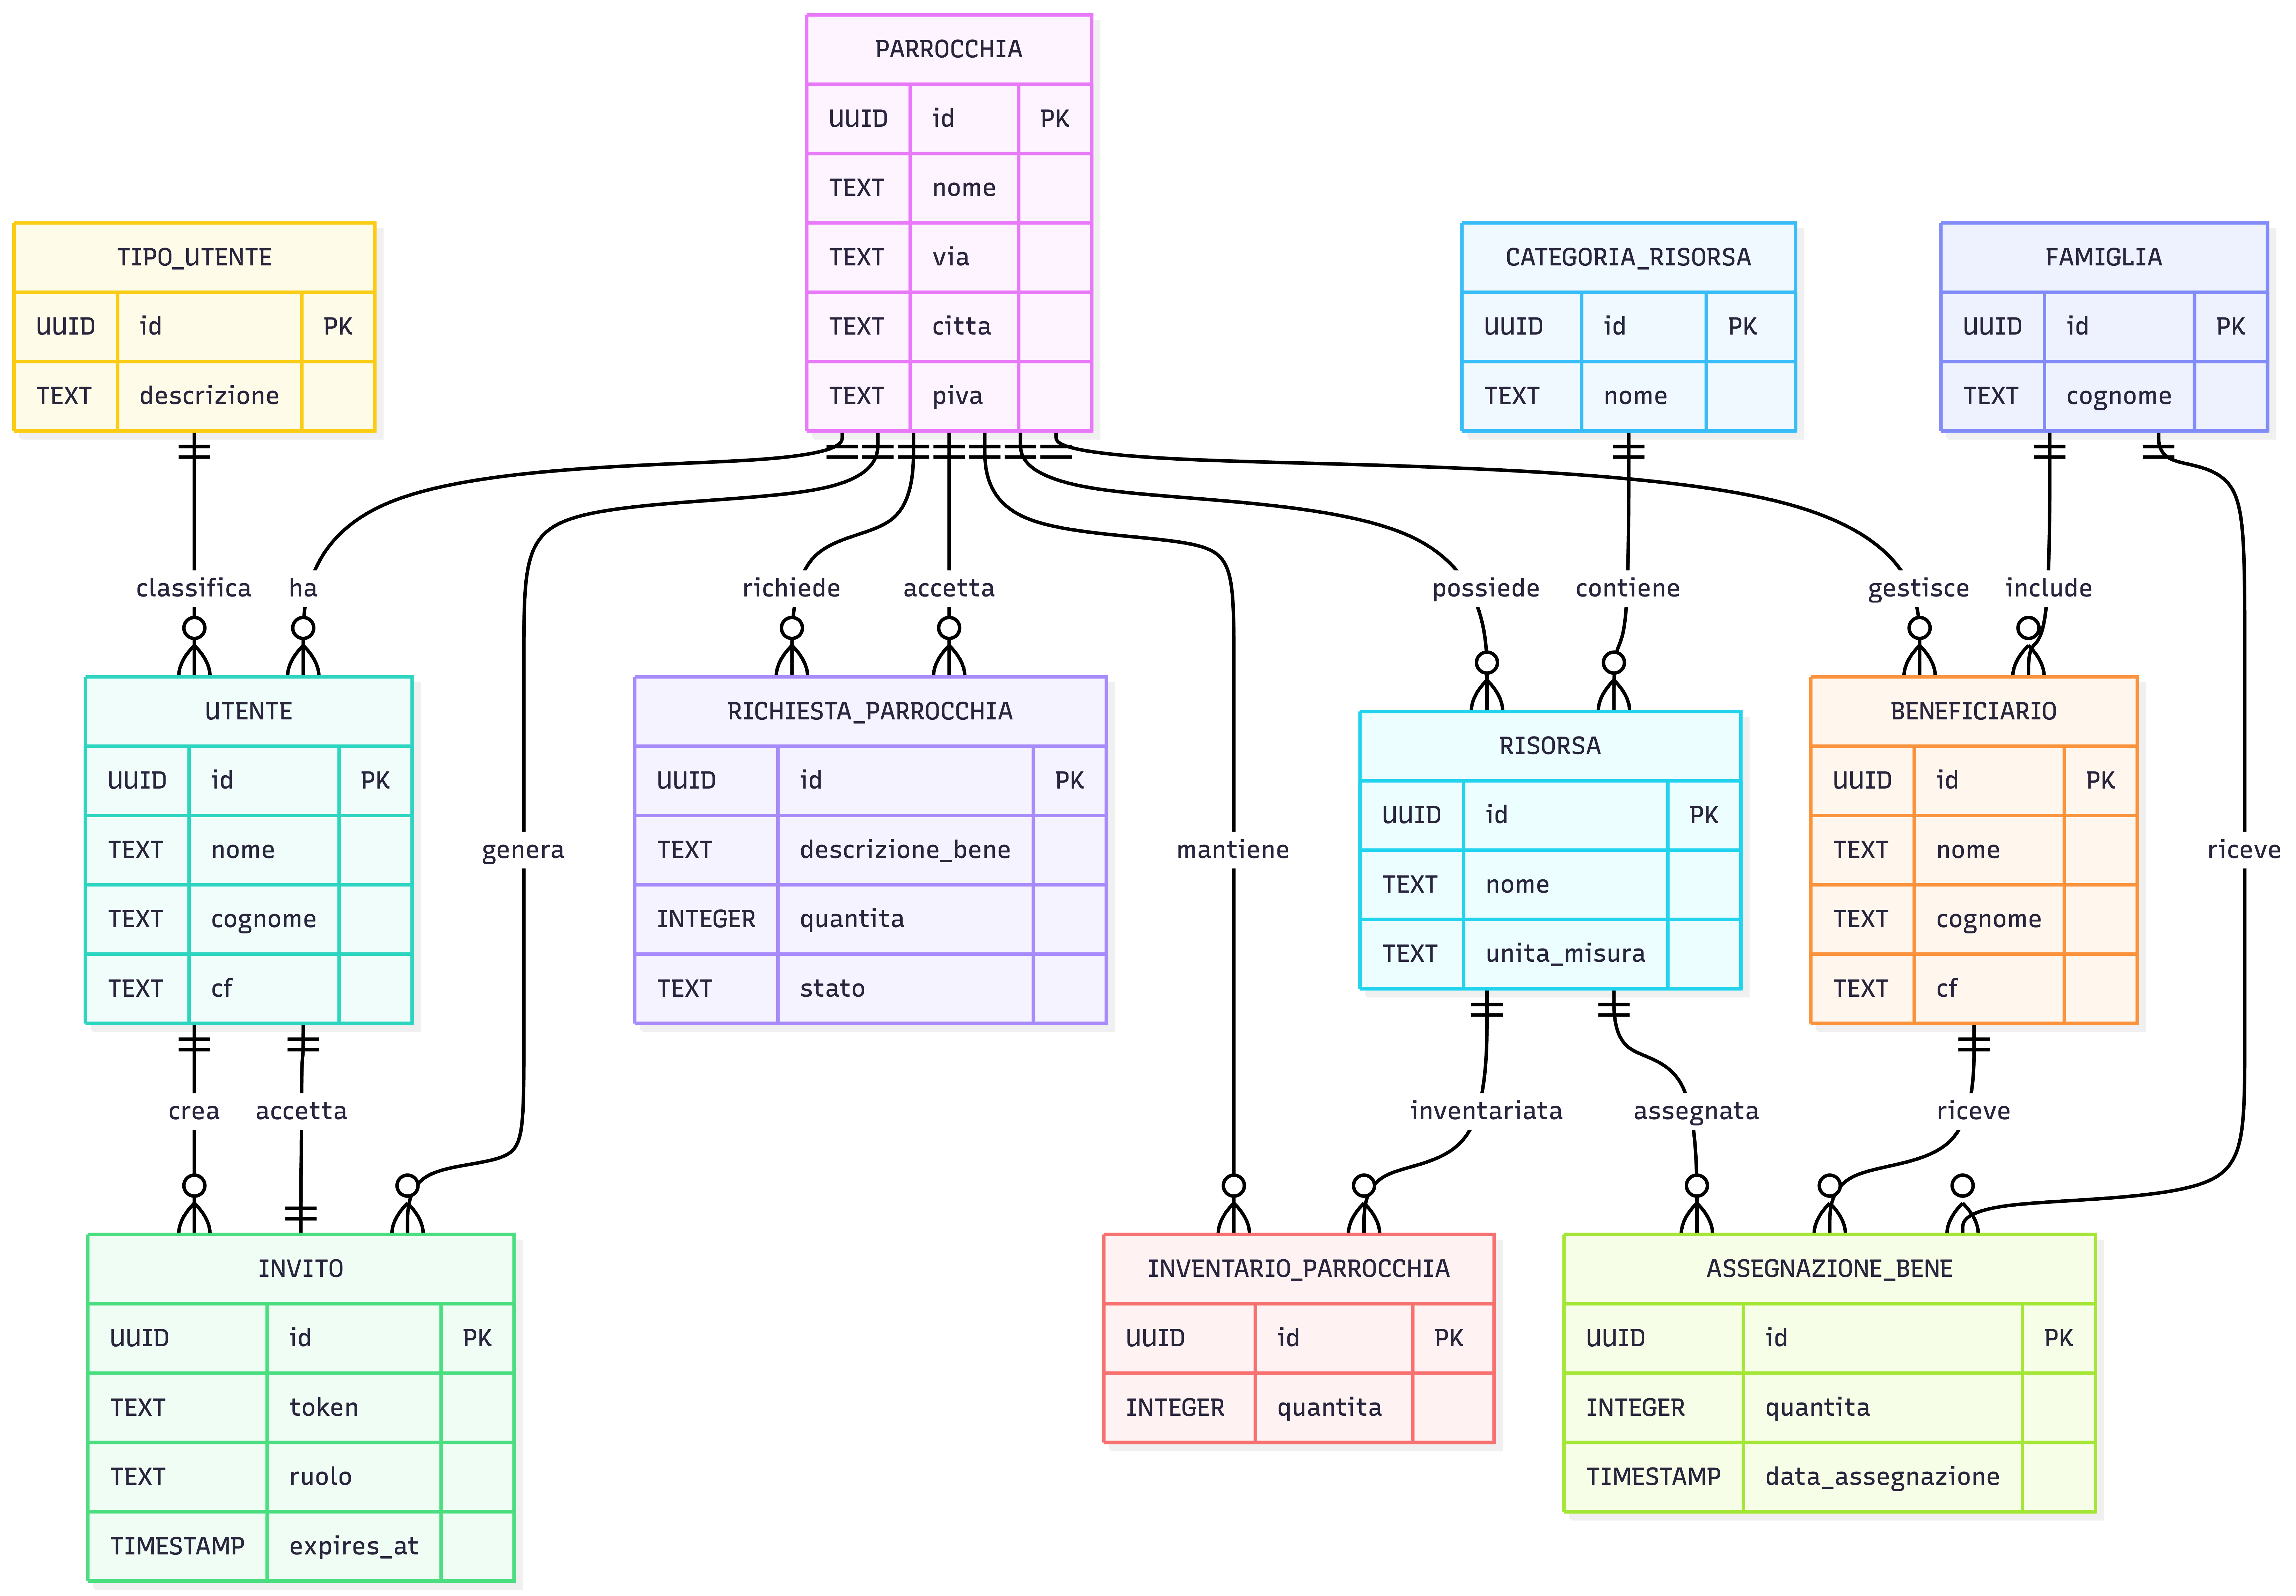
\includegraphics[width=0.9\textwidth]{er_schema.png}
\caption{Schema ER Database KARIS}
\end{figure}

\section{Relazioni}

\subsection{Relazioni Principali}

\begin{enumerate}[leftmargin=*]
\item \textbf{parrocchia $\leftrightarrow$ utente} (1:N)
   \begin{itemize}
   \item Una parrocchia può avere più utenti
   \item Un utente appartiene a una sola parrocchia
   \end{itemize}

\item \textbf{parrocchia $\leftrightarrow$ beneficiario} (1:N)
   \begin{itemize}
   \item Una parrocchia può avere più beneficiari
   \item Un beneficiario appartiene a una sola parrocchia
   \end{itemize}

\item \textbf{parrocchia $\leftrightarrow$ risorsa} (1:N)
   \begin{itemize}
   \item Una parrocchia può avere più risorse
   \item Una risorsa appartiene a una sola parrocchia
   \end{itemize}

\item \textbf{parrocchia $\leftrightarrow$ invito} (1:N)
   \begin{itemize}
   \item Una parrocchia può avere più inviti
   \item Un invito è valido per una sola parrocchia
   \end{itemize}

\item \textbf{parrocchia $\leftrightarrow$ richiesta\_parrocchia} (1:N come richiedente, N:1 come accettante)
   \begin{itemize}
   \item Una parrocchia può fare più richieste
   \item Una parrocchia può accettare più richieste
   \item Una richiesta è fatta da una parrocchia e può essere accettata da un'altra
   \end{itemize}

\item \textbf{tipo\_utente $\leftrightarrow$ utente} (1:N)
   \begin{itemize}
   \item Un tipo di utente può essere assegnato a più utenti
   \item Un utente ha un solo tipo
   \end{itemize}

\item \textbf{categoria\_risorsa $\leftrightarrow$ risorsa} (1:N)
   \begin{itemize}
   \item Una categoria può contenere più risorse
   \item Una risorsa appartiene a una sola categoria
   \end{itemize}

\item \textbf{famiglia $\leftrightarrow$ beneficiario} (1:N)
   \begin{itemize}
   \item Una famiglia può avere più beneficiari
   \item Un beneficiario appartiene a una sola famiglia
   \end{itemize}

\item \textbf{risorsa $\leftrightarrow$ inventario\_parrocchia} (1:N)
   \begin{itemize}
   \item Una risorsa può essere presente in più inventari
   \item Un record di inventario si riferisce a una sola risorsa
   \end{itemize}

\item \textbf{risorsa $\leftrightarrow$ assegnazione\_bene} (1:N)
   \begin{itemize}
   \item Una risorsa può essere assegnata più volte
   \item Un'assegnazione si riferisce a una sola risorsa
   \end{itemize}

\item \textbf{beneficiario $\leftrightarrow$ assegnazione\_bene} (N:1, opzionale)
   \begin{itemize}
   \item Un beneficiario può ricevere più assegnazioni
   \item Un'assegnazione può essere riferita a un solo beneficiario (o a una famiglia)
   \end{itemize}

\item \textbf{famiglia $\leftrightarrow$ assegnazione\_bene} (N:1, opzionale)
   \begin{itemize}
   \item Una famiglia può ricevere più assegnazioni
   \item Un'assegnazione può essere riferita a una sola famiglia (o a un beneficiario)
   \end{itemize}

\item \textbf{utente $\leftrightarrow$ invito} (1:N come creatore, N:1 come accettante)
   \begin{itemize}
   \item Un utente può creare più inviti
   \item Un utente può accettare un solo invito (vincolo UNIQUE su accepted\_by)
   \end{itemize}
\end{enumerate}

\section{Vincoli e Regole di Business}

\subsection{Vincoli di Integrità Referenziale}

\begin{itemize}
\item Tutte le foreign key sono definite con vincoli di integrità referenziale
\item Le chiavi primarie utilizzano UUID generati automaticamente
\end{itemize}

\subsection{Vincoli di Unicità}

\begin{itemize}
\item \texttt{utente.cf}: UNIQUE
\item \texttt{beneficiario.cf}: UNIQUE
\item \texttt{invito.token}: UNIQUE
\item \texttt{invito.accepted\_by}: UNIQUE (un utente può accettare un solo invito)
\end{itemize}

\subsection{Vincoli CHECK}

\begin{enumerate}
\item \textbf{invito.ruolo}: Deve essere 'volontario' o 'amministratore'
\item \textbf{richiesta\_parrocchia.stato}: Deve essere 'pending', 'accepted' o 'rejected'
\end{enumerate}

\subsection{Regole di Business}

\begin{enumerate}
\item \textbf{Assegnazione beni}: Un'assegnazione deve essere riferita O a un beneficiario O a una famiglia, ma non a entrambi contemporaneamente (vincolo implementato tramite CHECK constraint).

\item \textbf{Inviti}: 
   \begin{itemize}
   \item Gli inviti scadono dopo 7 giorni dalla creazione (default)
   \item Un utente può accettare un solo invito (vincolo UNIQUE su accepted\_by)
   \item Gli inviti possono essere revocati (campo revoked\_at)
   \end{itemize}

\item \textbf{Richieste tra parrocchie}:
   \begin{itemize}
   \item Lo stato iniziale è 'pending'
   \item Quando accettata, viene specificata la parrocchia\_accettante\_id
   \item Quando rifiutata, lo stato diventa 'rejected'
   \end{itemize}

\item \textbf{Inventario}: 
   \begin{itemize}
   \item La quantità può essere 0 o positiva
   \item Ogni combinazione parrocchia-risorsa può avere un solo record di inventario
   \end{itemize}

\item \textbf{Timestamp automatici}:
   \begin{itemize}
   \item \texttt{created\_at} viene impostato automaticamente alla creazione
   \item \texttt{updated\_at} viene aggiornato automaticamente per inventario\_parrocchia e richiesta\_parrocchia
   \end{itemize}
\end{enumerate}

\end{document}

